\documentclass[12pt, french]{report}
\usepackage[utf8]{inputenc}
\usepackage[T1]{fontenc}
\usepackage{babel}

%additional packages
\usepackage{amsmath}
\usepackage{graphicx}
\usepackage{caption}
\usepackage{subcaption}
\usepackage{longtable}
\graphicspath{{figures/}}
\usepackage[a4paper,width=160mm,top=25mm,bottom=25mm]{geometry}
\usepackage{titlesec}
\linespread{1.2}

\titleformat{\chapter}[hang]
  {\normalfont\LARGE\bfseries}
  {\color{blue!70!black}\chaptertitlename~\thechapter~:}
  {0.5em}
  {\color{black}}
\titlespacing*{\chapter}{0pt}{2ex}{1.5ex}

\usepackage{amsfonts,cite,array,multirow,graphicx,amsmath,amsthm,tabularx,setspace,amssymb,multirow}
\usepackage{tikz}

\newtheorem{theorem}{Theorem}
\newtheorem{lemma}{Lemma}
\usepackage{amsmath}
\usepackage{amsfonts}
\usepackage{amssymb}
\usepackage{bbm}
\usepackage{mathtools}
\usepackage{textcomp}
\usepackage{booktabs}
\usepackage{longtable}
\usepackage{multirow}
\usepackage{graphicx}
\usepackage{epigraph}
\usepackage{hyperref}
\usepackage{xcolor}
\usepackage{listings}
\usepackage{tcolorbox}

% Commande pour ajouter les chapitres non numérotés à la table des matières
\newcommand{\addstarredchapter}[1]{%
  \addcontentsline{toc}{chapter}{#1}%
}

\lstset{
  basicstyle=\ttfamily\small,
  backgroundcolor=\color{gray!10},
  frame=single,
  breaklines=true
}

\title{\Huge{Modélisation des comportements de santé par apprentissage automatique : régression, classification et clustering sur données synthétiques}}
\author{Ardacham Mahamat Teguene}
\date{Juin 2026}
\def\mytitle{Modélisation des comportements de santé par apprentissage automatique}
\def\myname{Ardacham Mahamat Teguene}
\def\degree{Master 1}
\def\mydegree{Mathématiques et Informatique Appliqués aux Sciences Humaines et Sociales}
\def\mysupervisor{}
\def\myrollno{}
\def\mydep{MIASHS}


\begin{document}

%Front Matter
\pagenumbering{roman}
 % !TEX root = manuscript.tex

% ── Logos ──────────────────────────────────────────────────────────────────
\begin{minipage}{.4\textwidth}
  \begin{center}
    \includegraphics[height=3cm]{logos/master.pdf}
  \end{center}
\end{minipage}%
\hspace{2cm}
\begin{minipage}{.4\textwidth}
  \begin{center}
    
\includegraphics[height=3cm]{logos/upv_new.png}
  \end{center}
\end{minipage}

\vspace{1.2cm}

% ── En-tête université / type de document ──────────────────────────────────
\begin{center}
  {\large Université de Montpellier Paul Valéry}\\[0.4cm]
  {\large\itshape Mémoire de fin de première année de Master}
\end{center}

\vspace{0.8cm}

% ── Titre ──────────────────────────────────────────────────────────────────
\begin{center}
  {\LARGE\bfseries Modélisation des comportements de santé\\[0.3cm]
  par apprentissage automatique~:\\[0.3cm]
  régression, classification et clustering\\[0.3cm]
  sur données synthétiques}
\end{center}

\vspace{2.5cm}

% ── Bloc identité ──────────────────────────────────────────────────────────
\begin{center}
  \renewcommand{\arraystretch}{1.8}
  \begin{tabular}{@{\hspace{1cm}}r@{\quad}l@{\hspace{1cm}}}
    \textbf{Étudiant}              & ARDACHAM Mahamat Teguene       \\
    \textbf{Formation}             & Master 1 MIASHS                \\
    \textbf{Tuteurs universitaires}& Sophie Lèbre \& Jérôme Pasquet \\
    \textbf{Année universitaire}   & 2025--2026                     \\
  \end{tabular}
\end{center}

\vfill

\begin{center}
  {\small Juin 2026}
\end{center}

\newpage

 \addstarredchapter{Remerciements}
 % !TEX root = ../manuscript.tex
{\vspace*{3cm}

\begin{center}
\Large\textbf{Remerciements}
\end{center}

\vspace{1cm}

Je tiens tout d'abord à remercier \textbf{Madame Sophie Lèbre} et \textbf{Monsieur Jérôme Pasquet}, mes tuteurs universitaires, pour leurs enseignements, leurs conseils tout au long de cette année, ainsi que pour la validation du sujet de ce mémoire.

Je remercie l'ensemble des enseignants du master \textbf{MIASHS} de l'Université de Montpellier Paul Valéry, dont les cours ont directement nourri ce projet~: \textbf{Maximilien Servagean}, \textbf{Catherine Trottier}, \textbf{Maïlis Amico}, \textbf{Arnaud Sallaberry}, \textbf{Sandra Bringay}, \textbf{Marine Demangeot} et~al. Leurs enseignements en machine learning, statistique, visualisation, optimisation, \ldots{} m'ont donné les outils nécessaires pour mener à bien cette analyse.

Je remercie également ma famille pour son soutien indéfectible tout au long de cette année, ainsi que mes amis et camarades de promotion, en particulier \textbf{ANZIZA Ahamada Madi}, pour les échanges, l'entraide et les moments partagés durant cette première année de master.

\vspace{1cm}
}
\newpage

 \addstarredchapter{Résumé}
 % !TEX root = ../manuscript.tex

\section*{Résumé}

Ce mémoire porte sur un projet de data science appliqué à la santé et aux modes de vie, avec pour objectif de modéliser des comportements à partir de données par apprentissage automatique. Le contexte médical s'appuie sur des seuils reconnus~: obésité (IMC $> 30$ selon l'OMS, Organisation Mondiale de la Santé~\cite{who2000}), hypercholestérolémie (cholestérol $> 200$~mg/dL selon le NCEP, National Cholesterol Education Program~\cite{ncep2002}), hypertension (pression systolique $\geq 140$~mmHg selon l'ESC, European Society of Cardiology~\cite{esc2018}). Le jeu de données utilisé est le \textit{Health \& Lifestyle Dataset}, un dataset synthétique de 100~000 individus décrits par 15 variables~: habitudes de vie (activité physique, sommeil, alimentation, tabagisme, alcool) et indicateurs biologiques (IMC, cholestérol, pression artérielle, fréquence cardiaque).

J'ai mis en place un pipeline complet selon la méthodologie CRISP-DM (Cross-Industry Standard Process for Data Mining)~\cite{chapman2000}, allant de l'exploration des données jusqu'à l'interprétabilité des modèles. L'analyse exploratoire et le feature engineering ont permis de préparer les données~: encodage des variables catégorielles, création de trois variables métier (score de style de vie composite, catégorie IMC, hypertension), standardisation. En \textbf{régression}, j'ai comparé six modèles (régression linéaire, Ridge, Lasso, ElasticNet, Random Forest, XGBoost) pour prédire le taux de cholestérol, avec tuning par \texttt{RandomizedSearchCV} et validation croisée K-Fold ($k=5$). Un data leakage a été détecté et corrigé sur la variable \texttt{hypercholesterol}~: le $R^2$ artificiel de 0.675 s'est réduit à $\approx 0$ après sa suppression. En \textbf{classification}, trois modèles ont prédit le risque de maladie (\texttt{disease\_risk}), avec deux stratégies de gestion du déséquilibre des classes comparées~: ajustement des poids (\texttt{class\_weight='balanced'}) et rééchantillonnage SMOTE~\cite{chawla2002}. En \textbf{clustering}, K-Means ($k=3$) a révélé trois profils biologiques et la CAH (liaison Ward, sous-échantillon de 5~000 individus) a isolé un groupe de fumeurs intenses hyperten dus~; les clusters ont été visualisés par ACP (24.3\% de variance en 2D). L'\textbf{interprétabilité} a été analysée via les coefficients des modèles linéaires, les feature importances et SHAP (utilisé ici comme complément visuel).

Le résultat principal est une \textbf{limite fondamentale du dataset synthétique}~: les variables ont été générées indépendamment, sans aucune relation causale. Aucun modèle n'a fait mieux qu'un prédicteur naïf ($R^2 \approx 0$, AUC $\approx 0.5$) — le Lasso annule les 16 coefficients, le Random Forest atteint $R^2 = -0.005$. La divergence entre les cinq méthodes d'interprétabilité le confirme. Ce n'est pas un échec méthodologique~: c'est la rigueur du pipeline qui a permis de le détecter. Ce travail est directement transposable à des données épidémiologiques réelles.

\bigskip
\noindent\textbf{Mots-clés~:} data science, santé, machine learning, régression, classification, clustering, interprétabilité, SHAP, SMOTE, données synthétiques, data leakage, CRISP-DM.

\newpage

 % !TEX root = ../manuscript.tex

\section*{Note sur l'utilisation de l'intelligence artificielle}
\addcontentsline{toc}{chapter}{Note sur l'utilisation de l'IA}

Dans le cadre de ce mémoire, j'ai eu recours à des outils d'intelligence artificielle générative --- principalement \textbf{Claude} (Anthropic) --- comme aide à la recherche et à la rédaction. Voici comment ces outils ont été utilisés concrètement~:

\begin{itemize}
  \item \textbf{Recherche bibliographique} : exploration et synthèse de la littérature sur les thématiques abordées (machine learning en santé, méthodes de régularisation, gestion du déséquilibre de classes, interprétabilité).
  \item \textbf{Structuration du document} : aide à l'organisation des chapitres et à la formulation des transitions.
  \item \textbf{Relecture et reformulation} : suggestions de reformulation pour améliorer la clarté des explications techniques.
  \item \textbf{Débogage et code} : aide au débogage des notebooks Python (scikit-learn, XGBoost, SHAP) et à la compilation \LaTeX.
\end{itemize}

L'ensemble du contenu scientifique --- choix des modèles, interprétation des résultats, analyse critique, conclusions --- a été compris, vérifié et validé par l'auteur. L'IA a servi d'outil d'assistance~; elle n'a pas remplacé le raisonnement ni le travail analytique qui constituent le c\oe ur de ce mémoire. Toutes les erreurs éventuelles restent de ma seule responsabilité.

\bigskip


\tableofcontents
\addstarredchapter{Liste des figures}
\listoffigures
\addstarredchapter{Liste des tableaux}
\listoftables

%Chapters
\clearpage
\pagenumbering{arabic}

\addstarredchapter{Introduction}
\addstarredchapter{Contexte}
% !TEX root = ../manuscript.tex
\chapter*{Introduction et contexte}

Aujourd'hui, les données de santé sont partout. Les montres connectées mesurent notre sommeil, les applications comptent nos pas, les bilans sanguins enregistrent notre cholestérol. On génère sans le savoir une quantité massive d'informations sur nos habitudes de vie. Mais avoir des données ne suffit pas : encore faut-il savoir les analyser, les comprendre, et en tirer des conclusions utiles.

C'est exactement ce que permet la data science. À l'intersection des mathématiques, de la statistique et de l'informatique, elle offre des outils concrets pour explorer des jeux de données complexes, construire des modèles prédictifs et surtout, expliquer ce qui se passe derrière les chiffres.

Ce mémoire présente un projet de data science appliqué à la santé et aux modes de vie, réalisé dans le cadre de la première année de master MIASHS. La question centrale qui guide l'ensemble du travail est la suivante :

\begin{center}
\textit{Quels facteurs du mode de vie influencent le plus l'état de santé d'un individu~--- et peut-on les identifier, les modéliser et les expliquer de manière rigoureuse~?}
\end{center}

\section*{La data science au service de la santé}

La santé publique constitue l'un des domaines d'application les plus prometteurs de la data science~\cite{obermeyer2016, rajpurkar2022}. L'apprentissage statistique permet aujourd'hui d'aborder des problèmes variés~: prédiction du risque de maladies chroniques, segmentation de populations selon leurs profils de santé, identification des facteurs de risque comportementaux~\cite{booth2012}.

Dans ce projet, l'objectif n'est pas seulement de prédire~--- c'est aussi et surtout de \textbf{comprendre}. Quand on prédit qu'une personne est à risque de maladie, il est crucial de pouvoir expliquer pourquoi~: est-ce à cause de son manque de sommeil~? De son cholestérol élevé~? De son inactivité physique~? Cette dimension explicative est au c\oe ur du travail présenté ici.

\section*{Présentation du jeu de données}

Le projet s'appuie sur le \textit{Health \& Lifestyle Dataset}, un jeu de données synthétique disponible sur Kaggle, composé de \textbf{100~000 individus} décrits par \textbf{15 variables}~:

\begin{itemize}
  \item \textbf{Habitudes de vie}~: \texttt{daily\_steps}, \texttt{sleep\_hours}, \texttt{water\_intake\_l}, \texttt{calories\_consumed}, \texttt{smoker}, \texttt{alcohol}.
  \item \textbf{Indicateurs biologiques}~: \texttt{bmi}, \texttt{resting\_hr}, \texttt{systolic\_bp}, \texttt{diastolic\_bp}, \texttt{cholesterol}.
  \item \textbf{Caractéristiques personnelles}~: \texttt{age}, \texttt{gender}, \texttt{family\_history}.
\end{itemize}

La variable cible principale est \texttt{disease\_risk}, un indicateur binaire (0/1) indiquant si un individu est considéré à risque de maladie. Bien que synthétique, ce dataset respecte des distributions statistiquement réalistes~\cite{chawla2002}, sans aucune contrainte éthique liée à des données personnelles réelles.

\section*{Lien avec la formation}

Ce projet est directement ancré dans les enseignements du master MIASHS~: réduction de dimension avec l'\textbf{ACP}, \textbf{régression linéaire et logistique}, \textbf{classification supervisée et non supervisée}, \textbf{régularisation et optimisation} (Ridge, Lasso, descente de gradient), et introduction au \textbf{deep learning}. Toutes ces notions sont mises en pratique ici de manière concrète, sur un problème à enjeu sociétal fort.

\section*{Objectifs du projet}

Le projet s'articule autour de quatre axes complémentaires~:

\begin{enumerate}
  \item \textbf{Analyse exploratoire}~--- comprendre la structure des données, les distributions, les corrélations, et formuler des hypothèses.
  \item \textbf{Régression}~--- prédire des indicateurs biologiques continus comme le taux de cholestérol.
  \item \textbf{Classification}~--- prédire le risque de maladie (\texttt{disease\_risk}) et comparer plusieurs algorithmes.
  \item \textbf{Clustering}~--- découvrir des profils types d'individus selon leur mode de vie.
\end{enumerate}


\chapter{État de l'art}
% !TEX root = ../manuscript.tex

\section{L'apprentissage automatique appliqué à la santé}

Ces dernières années, l'apprentissage automatique s'est imposé comme un outil incontournable dans le domaine de la santé. Des travaux pionniers comme ceux d'Obermeyer \& Emanuel~\cite{obermeyer2016} ont montré que les algorithmes de ML peuvent surpasser les méthodes statistiques classiques pour prédire des événements cliniques. Plus récemment, une revue publiée dans \textit{Nature Medicine}~\cite{rajpurkar2022} dresse un panorama des applications actuelles~: diagnostic médical assisté par IA, prédiction de risque de maladies chroniques, personnalisation des traitements.

Dans ce contexte, les jeux de données combinant indicateurs biologiques et habitudes de vie constituent un terrain d'étude particulièrement riche. L'idée centrale est que les maladies chroniques ne sont pas seulement le résultat de facteurs génétiques, mais résultent d'une accumulation de comportements quotidiens mesurables~\cite{booth2012}.

\section{Régression~: prédire des indicateurs biologiques}

La régression linéaire est l'une des méthodes les plus anciennes et les plus utilisées en statistique appliquée à la santé~\cite{james2021}. Pour pallier ses hypothèses fortes, des méthodes de \textbf{régression régularisée} ont été développées. La régression Ridge~\cite{hoerl1970} pénalise les coefficients trop grands via un terme $\lambda \|\mathbf{w}\|_2^2$, réduisant la variance du modèle. La régression Lasso~\cite{tibshirani1996} utilise une pénalisation $L_1$ qui force certains coefficients à zéro, réalisant ainsi une \textbf{sélection automatique de variables}.

Les méthodes ensemblistes comme les \textbf{forêts aléatoires}~\cite{breiman2001} et le \textbf{gradient boosting} (XGBoost~\cite{chen2016}) offrent des performances souvent supérieures sur des données tabulaires, en capturant les interactions non-linéaires entre variables.

\section{Classification~: prédire le risque de maladie}

La prédiction du risque de maladie est l'un des cas d'usage les plus étudiés en santé numérique. Des modèles de classification supervisée ont été appliqués avec succès à la prédiction du diabète de type 2~\cite{kavakiotis2017}, des maladies cardiovasculaires~\cite{mohan2019} ou encore de l'hypertension~\cite{olawade2023}.

Parmi les algorithmes les plus utilisés~:
\begin{itemize}
  \item La \textbf{régression logistique}~\cite{james2021}, modèle linéaire interprétable de référence.
  \item Les \textbf{forêts aléatoires}~\cite{breiman2001} et le \textbf{gradient boosting}~\cite{chen2016}, qui dominent les benchmarks sur données tabulaires.
\end{itemize}

Un point de vigilance important est le \textbf{déséquilibre des classes}~\cite{japkowicz2002}~: dans notre dataset, 75,2\% des individus sont sans risque contre seulement 24,8\% à risque. Un modèle naïf qui prédit toujours "sans risque" atteint déjà 75\% d'accuracy --- sans rien apprendre du tout.

Pour corriger ce biais, deux stratégies sont principalement utilisées. L'\textbf{ajustement des poids de classe} (\texttt{class\_weight='balanced'}) pénalise davantage les erreurs sur la classe minoritaire pendant l'entraînement, sans modifier les données. Le \textbf{SMOTE}~\cite{chawla2002} (\textit{Synthetic Minority Over-sampling Technique}) adopte une approche différente~: il crée synthétiquement de nouveaux exemples de la classe minoritaire en interpolant entre observations existantes. Pour un individu $x_i$ et l'un de ses $k$ plus proches voisins $x_{nn}$ dans la classe minoritaire~:

\begin{equation}
x_{\text{new}} = x_i + \lambda \cdot (x_{nn} - x_i), \quad \lambda \in [0, 1]
\end{equation}

Les deux stratégies sont appliquées et comparées dans ce projet. Comme on le verra, aucune ne parvient à améliorer significativement l'AUC~: cela confirme que le problème vient de l'absence de signal dans les données, et non du déséquilibre des classes.

\section{Clustering~: identifier des profils de mode de vie}

Le clustering vise à regrouper des individus similaires sans variable cible prédéfinie~\cite{macqueen1967}. Dans le domaine de la santé, cette approche est utilisée pour la \textbf{stratification de patients}~\cite{obermeyer2019}.

L'algorithme \textbf{K-Means}~\cite{macqueen1967} reste la méthode de référence. La \textbf{classification hiérarchique ascendante (CAH)} offre une représentation visuelle via le dendrogramme. L'évaluation d'un clustering se fait via le \textbf{coefficient de silhouette}~\cite{rousseeuw1987}~:

\begin{equation}
s(i) = \frac{b(i) - a(i)}{\max(a(i),\, b(i))}
\end{equation}

où $a(i)$ est la distance moyenne de l'observation $i$ aux autres points de son cluster, et $b(i)$ est la distance moyenne au cluster voisin le plus proche. Une valeur proche de 1 indique un clustering de qualité.

\section{Interprétabilité des modèles}

Un modèle performant ne suffit pas, notamment dans le domaine de la santé~: il faut aussi pouvoir \textbf{expliquer} ses prédictions~\cite{rudin2019}. Deux grandes familles d'approches se distinguent.

Les \textbf{modèles intrinsèquement interprétables} (régression linéaire, régression logistique, arbres de décision) permettent de lire directement les relations~: les coefficients d'une régression indiquent immédiatement le sens et l'amplitude de l'effet de chaque variable.

Les \textbf{méthodes post-hoc} sont appliquées \textit{après} l'entraînement, sur n'importe quel modèle --- y compris les boîtes noires comme Random Forest ou XGBoost. L'idée est simple~: ne pas sacrifier les performances prédictives pour avoir de l'interprétabilité, mais expliquer le modèle a posteriori. \textbf{SHAP}~\cite{lundberg2017} (\textit{SHapley Additive exPlanations}) est la méthode post-hoc la plus utilisée aujourd'hui. Issue de la théorie des jeux coopératifs, elle répond à la question~: \textit{quelle est la contribution équitable de chaque variable à cette prédiction précise ?} La valeur SHAP $\phi_j$ de la variable $j$ est~:

\begin{equation}
\phi_j = \sum_{S \subseteq F \setminus \{j\}} \frac{|S|!\,(|F|-|S|-1)!}{|F|!} \Bigl[ f(S \cup \{j\}) - f(S) \Bigr]
\end{equation}

où $F$ est l'ensemble des variables, $S$ un sous-ensemble ne contenant pas $j$, et $f(S)$ la prédiction du modèle avec uniquement les variables de $S$. Concrètement, pour chaque individu, SHAP produit un score signé par variable~: positif si la variable pousse vers le risque, négatif sinon.

Dans ce projet, SHAP est utilisé comme \textbf{complément visuel}, aux côtés des feature importances (Random Forest, XGBoost) et des coefficients de la régression logistique --- qui restent les interprétations principales.


\chapter{Données et analyse exploratoire}
% !TEX root = ../manuscript.tex
\minitoc
\newpage

\section{Analyse exploratoire des données (EDA)}

\subsection{Présentation générale du dataset}

Le jeu de données contient \textbf{100~000 observations} décrites par \textbf{15 variables} (l'identifiant \texttt{id} est exclu). On distingue trois types~: variables continues (âge, IMC, pas quotidiens, heures de sommeil, etc.), variables binaires (\texttt{smoker}, \texttt{alcohol}, \texttt{family\_history}, \texttt{disease\_risk}), et une variable catégorielle (\texttt{gender}). \textbf{Aucune valeur manquante} n'est détectée, ce qui s'explique par la nature synthétique des données.

\subsection{Statistiques descriptives}

Pour chaque variable continue $X = \{x_1, \ldots, x_n\}$ avec $n = 100\,000$, on calcule la moyenne et l'écart-type~\cite{saporta2011}~:

\begin{equation}
\bar{x} = \frac{1}{n}\sum_{i=1}^{n} x_i, \qquad
s = \sqrt{\frac{1}{n-1}\sum_{i=1}^{n}(x_i - \bar{x})^2}
\end{equation}

\begin{table}[h]
\centering
\caption{Statistiques descriptives des variables continues}
\label{tab:desc_stats}
\begin{tabular}{lrrrr}
\toprule
Variable & Moyenne & Écart-type & Min & Max \\
\midrule
\texttt{age} & 48.5 ans & 17.9 & 18 & 79 \\
\texttt{bmi} & 29.0 & 6.3 & 18.0 & 40.0 \\
\texttt{daily\_steps} & 10~480 & 5~484 & 1~000 & 19~999 \\
\texttt{sleep\_hours} & 6.5~h & 2.0 & 3.0 & 10.0 \\
\texttt{cholesterol} & 224.3~mg/dL & 43.3 & 150 & 299 \\
\texttt{systolic\_bp} & 134.6~mmHg & 26.0 & 90 & 179 \\
\texttt{resting\_hr} & 74.5~bpm & 14.4 & 50 & 99 \\
\bottomrule
\end{tabular}
\end{table}

\begin{quote}
\textbf{Interprétation~:} Un IMC moyen de 29 se situe en limite de surpoids selon la classification OMS, qui fixe le seuil à 25~kg/m²~\cite{who2000}. Le taux moyen de cholestérol à 224~mg/dL dépasse le seuil de 200~mg/dL recommandé par le NCEP~\cite{ncep2002}.
\end{quote}

\subsection{Distribution des variables}

Le coefficient d'asymétrie (skewness) mesure la symétrie d'une distribution~\cite{saporta2011}~:

\begin{equation}
\text{Skew}(X) = \frac{1}{n}\sum_{i=1}^{n}\left(\frac{x_i - \bar{x}}{s}\right)^3
\end{equation}

Toutes les variables continues affichent un skewness inférieur à $|0.02|$~: distributions \textbf{quasi-uniformes}, caractéristique typique des données synthétiques générées par tirage aléatoire~\cite{chawla2002}.

La variable cible présente un \textbf{déséquilibre}~: 75~179 individus (75.2\%) sans risque contre 24~821 (24.8\%) à risque. Ce déséquilibre, connu sous le nom de \textit{class imbalance problem}~\cite{japkowicz2002}, justifie l'utilisation du F1-score, de la précision et du rappel plutôt que la seule accuracy~\cite{sokolova2009}.

\subsection{Analyse des corrélations}

Le coefficient de corrélation de Pearson entre deux variables $X$ et $Y$~\cite{pearson1895}~:

\begin{equation}
r_{XY} = \frac{\sum_{i=1}^{n}(x_i - \bar{x})(y_i - \bar{y})}
{\sqrt{\sum_{i=1}^{n}(x_i-\bar{x})^2 \cdot \sum_{i=1}^{n}(y_i-\bar{y})^2}}
\end{equation}

\begin{quote}
\textbf{Résultat central~:} Les corrélations entre toutes les variables du dataset sont inférieures à $|0.01|$. La variable la plus corrélée avec \texttt{disease\_risk} est \texttt{resting\_hr} avec $r = 0.005$ --- statistiquement non significatif. Cela s'explique par la nature synthétique du dataset~: la variable cible semble avoir été générée indépendamment des autres variables. Ce constat justifie l'exploration de méthodes non-linéaires~\cite{breiman2001}.
\end{quote}

\subsection{Bilan de l'EDA}

\begin{table}[h]
\centering
\caption{Bilan de l'analyse exploratoire}
\label{tab:eda_bilan}
\begin{tabular}{lll}
\toprule
Point & Constat & Implication \\
\midrule
Valeurs manquantes & Aucune & Pas de preprocessing nécessaire \\
Distributions & Quasi-uniformes & Pas de transformation logarithmique \\
Outliers & Aucun (méthode IQR) & Pas de traitement nécessaire \\
Corrélations & Quasi-nulles ($< 0.01$) & Privilégier modèles non-linéaires \\
Classe cible & Déséquilibrée (75/25) & Utiliser F1-score, AUC-ROC \\
\bottomrule
\end{tabular}
\end{table}

\section{Feature Engineering et préparation des données}

\subsection{Encodage des variables catégorielles}

La variable \texttt{gender} est encodée en variable binaire~\cite{geron2019}~:

\begin{equation}
\texttt{gender\_enc} = \begin{cases} 1 & \text{si Male} \\ 0 & \text{si Female} \end{cases}
\end{equation}

La colonne \texttt{id} est supprimée~: identifiant technique sans pouvoir prédictif. La variable \texttt{hypercholesterol} ($= 1$ si \texttt{cholesterol} $> 200$) est créée pour le clustering mais \textbf{exclue de la régression} car directement dérivée de la variable cible~--- c'est un \textit{data leakage}~\cite{kaufman2012}.

\subsection{Création de nouvelles variables}

Trois nouvelles variables sont construites à partir de connaissances métier~\cite{kuhn2019}~:

\textbf{Hypertension} selon les seuils ESC~\cite{esc2018}~:
\begin{equation}
\texttt{hypertension} = \begin{cases} 1 & \text{si } \texttt{systolic\_bp} \geq 140 \text{ ou } \texttt{diastolic\_bp} \geq 90 \\ 0 & \text{sinon} \end{cases}
\end{equation}

\textbf{Catégories IMC} selon la classification OMS~\cite{who2000}~:
\begin{equation}
\texttt{bmi\_cat} = \begin{cases} 0 & \texttt{bmi} < 18.5\ \text{(sous-poids)} \\ 1 & 18.5 \leq \texttt{bmi} < 25\ \text{(normal)} \\ 2 & 25 \leq \texttt{bmi} < 30\ \text{(surpoids)} \\ 3 & \texttt{bmi} \geq 30\ \text{(obèse)} \end{cases}
\end{equation}

\textbf{Score de style de vie} (variables normalisées par leur maximum)~:
\begin{equation}
\texttt{lifestyle\_score} = \frac{\texttt{daily\_steps}}{\max} + \frac{\texttt{sleep\_hours}}{\max} + \frac{\texttt{water\_intake\_l}}{\max} - \texttt{smoker} - \texttt{alcohol} - \frac{\texttt{bmi}}{\max} - \frac{\texttt{calories\_consumed}}{\max}
\end{equation}

\subsection{Mise à l'échelle}

Deux méthodes de mise à l'échelle sont appliquées selon le contexte~\cite{hastie2009}~:

\textbf{Standardisation (z-score)} pour les modèles linéaires et SVM~:
\begin{equation}
z_i = \frac{x_i - \bar{x}}{s}
\end{equation}

\textbf{Normalisation min-max} pour les algorithmes de distance (K-Means)~:
\begin{equation}
x_i^{\text{norm}} = \frac{x_i - x_{\min}}{x_{\max} - x_{\min}}
\end{equation}

\subsection{Dataset final}

Après preprocessing, le dataset contient \textbf{16 variables explicatives} couvrant les dimensions démographiques, les habitudes de vie, les indicateurs biologiques et les variables construites.


\chapter{Modélisation supervisée}
% !TEX root = ../manuscript.tex
\minitoc
\newpage

\section{Régression~: prédire le taux de cholestérol}

\subsection{Objectif et variable cible}

L'objectif est de prédire le taux de cholestérol (\texttt{cholesterol}, en mg/dL) à partir des habitudes de vie et indicateurs biologiques. Ce choix est médicalement motivé~: le cholestérol est un facteur de risque cardiovasculaire reconnu~\cite{ncep2002}.

\textbf{Note sur le data leakage~:} la variable \texttt{hypercholesterol} ($= 1$ si cholestérol $> 200$) est directement dérivée de la variable cible. L'inclure comme feature constitue un \textit{data leakage}~\cite{kaufman2012} qui gonfle artificiellement le R² à 0.675. Une fois retirée, le R² chute à $\approx 0$ pour tous les modèles, confirmant l'absence de signal prédictif.

\subsection{Protocole expérimental}

\textbf{Split 80/20}~: 80~000 individus en entraînement, 20~000 en test (\texttt{random\_state=42}). Le jeu de test n'intervient qu'à l'évaluation finale~\cite{james2021}.

\textbf{Validation croisée K-Fold ($k=5$)}~\cite{hastie2009}~: le jeu d'entraînement est découpé en 5 plis. Le score moyen est estimé par~:
\begin{equation}
\text{CV-score} = \frac{1}{k}\sum_{i=1}^{k} \text{score}_i, \quad k=5
\end{equation}

\textbf{Métriques d'évaluation}~\cite{james2021}~:
\begin{align}
R^2 &= 1 - \frac{\sum(y_i - \hat{y}_i)^2}{\sum(y_i - \bar{y})^2} \\
\text{RMSE} &= \sqrt{\frac{1}{n}\sum(y_i - \hat{y}_i)^2} \\
\text{MAE} &= \frac{1}{n}\sum|y_i - \hat{y}_i|
\end{align}

\subsection{Modèles et justification}

\textbf{Régression linéaire (baseline)}~: référence obligatoire. Si les autres modèles ne font pas mieux, la complexité ajoutée n'est pas justifiée~\cite{james2021}.

\textbf{Ridge (régularisation $L_2$)}~\cite{hoerl1970}~:
\begin{equation}
\mathcal{L}_{\text{Ridge}} = \sum(y_i - \hat{y}_i)^2 + \lambda\sum_j w_j^2
\end{equation}

\textbf{Lasso (régularisation $L_1$)}~\cite{tibshirani1996}~: force certains coefficients à zéro, réalisant une \textbf{sélection automatique de variables}~:
\begin{equation}
\mathcal{L}_{\text{Lasso}} = \sum(y_i - \hat{y}_i)^2 + \lambda\sum_j |w_j|
\end{equation}

\textbf{ElasticNet}~\cite{hastie2009}~: combine $L_1$ et $L_2$ via un paramètre $\rho \in [0,1]$~:
\begin{equation}
\mathcal{L}_{\text{EN}} = \sum(y_i - \hat{y}_i)^2 + \lambda\left[\rho\sum_j|w_j| + \frac{1-\rho}{2}\sum_j w_j^2\right]
\end{equation}

\textbf{Random Forest}~\cite{breiman2001}~: ensemble de $B$ arbres avec prédiction par moyenne~:
\begin{equation}
\hat{y} = \frac{1}{B}\sum_{b=1}^{B} T_b(\mathbf{x})
\end{equation}
Paramètres~: \texttt{max\_depth=15}, \texttt{max\_samples=0.5}, \texttt{n\_jobs=-1} pour éviter les entraînements de plusieurs heures observés avec les paramètres par défaut.

\textbf{XGBoost}~\cite{chen2016}~: gradient boosting séquentiel avec régularisation intégrée~:
\begin{equation}
\hat{y}^{(t)} = \hat{y}^{(t-1)} + \eta \cdot T_t(\mathbf{x})
\end{equation}

\textbf{Tuning par RandomizedSearchCV}~\cite{bergstra2012}~: tire aléatoirement \texttt{n\_iter=20} combinaisons dans l'espace des hyperparamètres, divisant le temps de calcul par rapport à GridSearch tout en explorant suffisamment l'espace.

\subsection{Résultats et analyse critique}

\begin{table}[h]
\centering
\caption{Résultats de régression (variable cible~: \texttt{cholesterol})}
\label{tab:regression_results}
\begin{tabular}{lrrrr}
\toprule
Modèle & $R^2$ & RMSE (mg/dL) & MAE (mg/dL) & CV-$R^2$ \\
\midrule
LinearRegression (baseline) & 0.0001 & 43.33 & 37.59 & $\approx 0$ \\
Ridge ($\alpha=7197$, tuné) & 0.0001 & 43.33 & 37.59 & $\approx 0$ \\
Lasso ($\alpha=9.54$, tuné) & $\approx 0$ & 43.33 & 37.60 & $\approx 0$ \\
ElasticNet & 0.0001 & 43.33 & 37.60 & $\approx 0$ \\
Random Forest (tuné) & $\approx 0$ & 43.34 & 37.61 & $\approx 0$ \\
XGBoost (tuné) & 0.0001 & 43.33 & 37.59 & $\approx 0$ \\
\bottomrule
\end{tabular}
\end{table}

\begin{quote}
\textbf{Analyse critique~:} Aucun modèle ne réussit à prédire le taux de cholestérol ($R^2 \approx 0$). Le Lasso, en fixant tous ses coefficients à zéro, confirme formellement l'absence de signal prédictif linéaire. Ce résultat illustre une \textbf{limite fondamentale du dataset synthétique}~: les variables ont été générées indépendamment, sans relations causales réalistes. Dans des données réelles, l'alimentation, l'activité physique et le tabagisme influencent significativement le cholestérol~\cite{booth2012} --- mais cette relation n'existe pas ici. La valeur de cet exercice réside dans la \textbf{démonstration méthodologique}~: pipeline complet, détection de data leakage, comparaison de 6 modèles avec tuning.
\end{quote}

\section{Classification~: prédire le risque de maladie}

\subsection{Objectif et contexte}

L'objectif est de prédire si un individu est à risque de maladie (\texttt{disease\_risk} = 1) ou non (\texttt{disease\_risk} = 0). Le dataset présente un \textbf{déséquilibre de classes}~: 75.2\% sans risque, 24.8\% à risque~\cite{japkowicz2002}.

\subsection{Protocole expérimental}

\textbf{Split stratifié 80/20}~: le paramètre \texttt{stratify=y} maintient le ratio 75.2/24.8 dans les deux ensembles~\cite{james2021}.

\textbf{Stratified K-Fold ($k=5$)}~: maintient le ratio de classes dans chaque fold~\cite{japkowicz2002}.

\textbf{Gestion du déséquilibre}~\cite{japkowicz2002}~:
\begin{equation}
w_k = \frac{n}{K \cdot n_k}
\end{equation}
via \texttt{class\_weight='balanced'} (Logistic Regression, Random Forest) et \texttt{scale\_pos\_weight=3} (XGBoost).

\subsection{Métriques d'évaluation}

\begin{align}
\text{Précision} &= \frac{TP}{TP+FP}, \quad \text{Rappel} = \frac{TP}{TP+FN} \\
\text{F1-score} &= \frac{2 \times \text{Précision} \times \text{Rappel}}{\text{Précision} + \text{Rappel}}
\end{align}

La courbe \textbf{ROC} trace le taux de vrais positifs en fonction du taux de faux positifs. L'\textbf{AUC-ROC}~\cite{james2021} mesure la capacité de discrimination~: AUC = 0.5 équivaut à un tirage aléatoire.

\textbf{Note sur le SVM~:} sa complexité en $\mathcal{O}(n^2)$ à $\mathcal{O}(n^3)$~\cite{cortes1995} le rend impraticable sur 100~000 observations sans infrastructure dédiée. Un test sur 5~000 individus a confirmé des performances similaires aux autres modèles.

\subsection{Résultats}

\begin{table}[h]
\centering
\caption{Résultats de classification (variable cible~: \texttt{disease\_risk})}
\label{tab:classif_results}
\begin{tabular}{lrrrrr}
\toprule
Modèle & Accuracy & Précision & Rappel & F1 & AUC-ROC \\
\midrule
Naïf (tout à 0) & 0.752 & --- & 0.000 & 0.000 & 0.500 \\
Logistic Regression & 0.498 & 0.249 & 0.509 & 0.335 & 0.499 \\
Random Forest & 0.568 & 0.245 & 0.355 & 0.290 & 0.494 \\
XGBoost & 0.531 & 0.248 & 0.436 & 0.316 & 0.499 \\
\bottomrule
\end{tabular}
\end{table}

\begin{quote}
\textbf{Analyse critique~:} L'\textbf{AUC-ROC~$\approx$~0.5} pour tous les modèles signifie qu'ils n'ont aucun pouvoir discriminant réel~\cite{james2021}~--- équivalent à un tirage à pile ou face. La comparaison avec le modèle naïf est instructive~: avec \texttt{class\_weight='balanced'}, les modèles augmentent leur rappel mais au prix d'une accuracy inférieure à 50\%. Cela démontre concrètement pourquoi l'accuracy seule est trompeuse sur un dataset déséquilibré~\cite{sokolova2009}~: un modèle à 75\% d'accuracy qui ne prédit jamais de risque est inutile en pratique. Les importances de features sont uniformément distribuées, confirmant qu'aucune variable n'est réellement prédictive de \texttt{disease\_risk}.
\end{quote}


\chapter{Clustering et interprétabilité}
% !TEX root = ../manuscript.tex

\section{Clustering~: identifier des profils de mode de vie}

\subsection{Objectif}

Le clustering est une méthode d'\textbf{apprentissage non supervisé}~: il n'y a pas de variable cible. L'objectif est de regrouper les individus selon leur similarité pour identifier des \textbf{profils types de mode de vie}~\cite{macqueen1967}. La variable \texttt{disease\_risk} est exclue du clustering.

\subsection{Préparation des données}

Les 15 variables explicatives sont standardisées (z-score) avant d'appliquer les algorithmes. K-Means et CAH reposent sur la \textbf{distance euclidienne}~\cite{macqueen1967}~: sans standardisation, \texttt{daily\_steps} (valeurs jusqu'à 20~000) dominerait mécaniquement \texttt{sleep\_hours} (3 à 10), et le clustering serait réduit à une partition par cette seule variable. Le z-score garantit une contribution équitable de chacune des 15 dimensions~\cite{hastie2009}.

La CAH étant de complexité $\mathcal{O}(n^2)$ (voir note sur le SVM au chapitre~3), elle est appliquée sur un sous-échantillon aléatoire de \textbf{5~000 individus} pour rester dans des temps de calcul raisonnables.

\subsection{Sélection du nombre de clusters}

\textbf{Méthode du coude}~: on trace l'\textbf{inertie intra-cluster} $W(k)$ en fonction de $k$. L'inertie mesure la dispersion totale à l'intérieur des clusters~:
\begin{equation}
W(k) = \sum_{j=1}^{k}\sum_{\mathbf{x} \in C_j}\|\mathbf{x} - \boldsymbol{\mu}_j\|^2
\end{equation}
où $C_j$ désigne le $j$-ème cluster et $\boldsymbol{\mu}_j$ son centroïde (vecteur des moyennes). Plus $k$ augmente, plus l'inertie diminue --- mais à partir d'un certain $k$, le gain devient marginal~: c'est le "coude" de la courbe, au-delà duquel ajouter des clusters ne compense plus la complexité.

\textbf{Coefficient de silhouette}~\cite{rousseeuw1987}~: défini au chapitre~1, il mesure la qualité de séparation des clusters. Pour rappel~:
\begin{equation}
s(i) = \frac{b(i) - a(i)}{\max(a(i),\, b(i))}
\end{equation}
où $a(i)$ est la distance moyenne de l'individu $i$ aux autres membres de son cluster, et $b(i)$ la distance moyenne au cluster voisin le plus proche. Une valeur proche de 1 indique une bonne séparation.

\begin{table}[h]
\centering
\caption{Inertie et silhouette selon $k$ (K-Means)}
\label{tab:kmeans_k}
\begin{tabular}{rrr}
\toprule
$k$ & Inertie & Silhouette \\
\midrule
2 & 1~346~768 & 0.0979 \\
\textbf{3} & \textbf{1~238~076} & \textbf{0.1030} \\
4 & 1~188~303 & 0.0967 \\
5 & 1~152~260 & 0.0886 \\
10 & 1~031~548 & 0.0744 \\
\bottomrule
\end{tabular}
\end{table}

$k=3$ maximise la silhouette et correspond au coude de la courbe d'inertie. \textbf{$k=3$ est retenu.}

\begin{figure}[h]
\centering
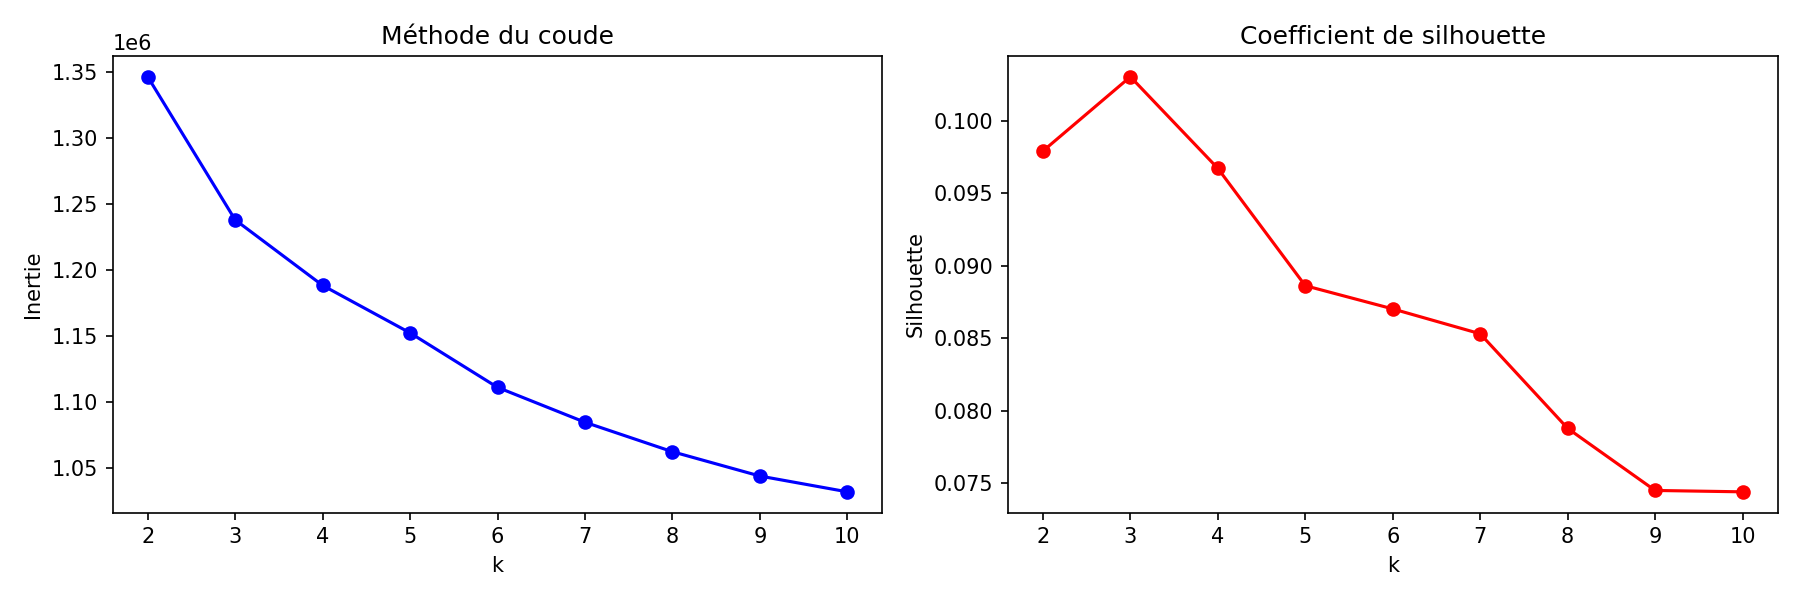
\includegraphics[width=0.85\textwidth]{kmeans_selection_k.png}
\caption{Inertie intra-cluster et coefficient de silhouette selon $k$ (K-Means)}
\label{fig:kmeans_k}
\end{figure}

\subsection{K-Means}

L'algorithme K-Means~\cite{macqueen1967} alterne affectation au centroïde le plus proche et mise à jour des centroïdes~: $\boldsymbol{\mu}_j = \frac{1}{|C_j|}\sum_{\mathbf{x} \in C_j} \mathbf{x}$, jusqu'à convergence.

\begin{table}[h]
\centering
\caption{Profils des clusters K-Means ($k=3$)}
\label{tab:kmeans_profiles}
\begin{tabular}{llrrl}
\toprule
Cluster & Taille & IMC moyen & Syst. (mmHg) & Profil \\
\midrule
0 & 32~754 & 35.0 (obèse)    & 142 (hypertendu)  & Obèse hypertendu \\
1 & 27~673 & 29.1 (surpoids) & 115 (normotendu)  & Surpoids normotendu \\
2 & 39~573 & 24.0 (normal)   & 142 (hypertendu)  & Poids normal hypertendu \\
\bottomrule
\end{tabular}
\end{table}

\begin{quote}
\textbf{Interprétation~:} K-Means partitionne la population selon l'\textbf{IMC} et la \textbf{pression artérielle systolique}. Ce résultat s'explique par la sensibilité de K-Means aux variables à grande variance~: dans notre dataset, \texttt{bmi} (écart-type = 6.3) et \texttt{systolic\_bp} (écart-type = 26.0) ont les dispersions les plus larges après standardisation, ce qui les rend naturellement "dominantes" pour la distance euclidienne. Le cluster~1 regroupe les individus les plus sains (surpoids mais normotendus), tandis que les clusters~0 et~2 correspondent à deux profils à risque cardiovasculaire distincts selon la classification OMS~\cite{who2000} et ESC~\cite{esc2018}.
\end{quote}

\subsection{Classification Hiérarchique Ascendante (CAH)}

La CAH construit un \textbf{dendrogramme} en fusionnant progressivement les clusters les plus proches. Au départ, chaque individu est son propre cluster~; à chaque étape, on fusionne les deux clusters dont la fusion est la "moins coûteuse"~\cite{hastie2009}.

La \textbf{méthode de liaison Ward} définit le coût de fusion de $A$ et $B$ comme l'augmentation de variance intra-cluster~:
\begin{equation}
\Delta(A, B) = \frac{|A|\cdot|B|}{|A|+|B|}\|\boldsymbol{\mu}_A - \boldsymbol{\mu}_B\|^2
\end{equation}
Ward minimise ce coût à chaque étape, favorisant des clusters \textbf{compacts et équilibrés}~--- d'où sa sensibilité aux sous-groupes comportementaux homogènes dans nos données.

\begin{table}[h]
\centering
\caption{Profils des clusters CAH ($k=3$, $n=5~000$)}
\label{tab:cah_profiles}
\begin{tabular}{llrrl}
\toprule
Cluster & Taille & Fumeurs & Syst. (mmHg) & Profil \\
\midrule
0 & 2~928 & 2\%           & 142 & Non-fumeurs hyperten dus \\
1 & 1~407 & 18\%          & 115 & Fumeurs modérés, normotendus \\
2 &   665 & \textbf{100\%}& 142 & Fumeurs intenses, hyperten dus \\
\bottomrule
\end{tabular}
\end{table}

\begin{quote}
\textbf{Interprétation~:} La CAH isole un \textbf{cluster de fumeurs intenses} (100\% de fumeurs + hypertendus). Ce résultat s'explique par la nature de l'algorithme~: Ward cherche des sous-groupes \textit{homogènes}, y compris sur des variables binaires comme \texttt{smoker}. K-Means, guidé par les grandes variances numériques, n'aurait pas isolé ce groupe de 665 individus --- il les aurait dilués dans les clusters dominés par l'IMC et la pression. Les deux méthodes sont donc \textbf{complémentaires}~: K-Means donne une vue globale par dimensions biologiques continues, la CAH révèle des sous-groupes comportementaux fins. Le profil tabagisme + hypertension est un double facteur de risque cardiovasculaire bien documenté~\cite{booth2012}.
\end{quote}

\subsection{Évaluation et visualisation}

\textbf{Visualisation par ACP (Analyse en Composantes Principales).} Nos données vivent dans un espace à 15 dimensions~: il est impossible de les représenter directement. L'ACP projette ces 15 dimensions sur les 2 axes qui capturent le maximum de variance, permettant une visualisation 2D des clusters. Les deux premières composantes expliquent \textbf{24.3\%} de la variance totale~: la projection 2D "voit" seulement 24.3\% de l'information originale. Si les clusters semblent peu séparés sur le graphique, ce n'est pas la preuve qu'ils n'existent pas --- ils se distinguent dans les 15 dimensions d'origine, pas dans la réduction 2D. Avec 15 variables quasi-indépendantes (confirmé par l'EDA), aucune direction ne concentre beaucoup de variance~: 24.3\% en 2D est donc attendu.

\textbf{Pourquoi les clusters ont-ils une forme rectangulaire dans la projection ACP~?} Sur le graphique ACP (figure~\ref{fig:kmeans_pca}), les clusters apparaissent comme des \textbf{blocs rectangulaires} plutôt que des nuages sphériques --- résultat directement lié à la nature des variables du dataset.

La première composante principale (PC1, axe horizontal) est fortement influencée par \texttt{bmi\_cat}, une variable ordinale à \textbf{4 valeurs discrètes} (0 = sous-poids, 1 = normal, 2 = surpoids, 3 = obèse). Cette discrétisation crée des \textbf{colonnes verticales}~: les individus s'alignent en 4 bandes distinctes plutôt que de se répartir continûment sur l'axe. La deuxième composante (PC2, axe vertical) est dominée par \texttt{hypertension}, une variable \textbf{binaire} (0 ou 1)~: une variable binaire ne peut prendre que deux valeurs, ce qui produit un \textbf{saut net haut/bas} dans la projection, divisant les individus entre normotendus (bas) et hypertendus (haut).

Par ailleurs, les distributions quasi-uniformes de toutes les variables continues (chapitre~2) créent des nuages de points dispersés sans gradient de densité visible~: les points se répartissent uniformément au lieu de former des ellipses denses au centre. Le résultat final est une grille de rectangles dont la forme reflète la structure discrète du dataset plutôt qu'une vraie géométrie en clusters.

\textbf{Indice de Davies-Bouldin~\cite{davies1979}.} Cet indice mesure la qualité du clustering en calculant, pour chaque cluster $i$, le ratio entre la dispersion interne et la distance entre centroïdes~:
\begin{equation}
DB = \frac{1}{k}\sum_{i=1}^{k}\max_{j \neq i}\left(\frac{\sigma_i + \sigma_j}{d(\boldsymbol{\mu}_i, \boldsymbol{\mu}_j)}\right)
\end{equation}
où $\sigma_i$ est la dispersion moyenne des points du cluster $i$ autour de son centroïde, et $d(\boldsymbol{\mu}_i, \boldsymbol{\mu}_j)$ la distance entre les centroïdes $i$ et $j$. \textbf{Un DB proche de 0 est idéal}~: les clusters sont compacts (faible $\sigma$) et bien séparés (grande distance). Un DB élevé indique des clusters éparpillés ou trop proches les uns des autres. Contrairement à la silhouette qui évalue chaque point individuellement, Davies-Bouldin évalue chaque paire de clusters~: les deux métriques sont complémentaires.

\begin{table}[h]
\centering
\caption{Comparaison K-Means vs CAH}
\label{tab:clustering_eval}
\begin{tabular}{lrrl}
\toprule
Métrique & K-Means & CAH & Interprétation \\
\midrule
Silhouette      & 0.103 & 0.105 & Faible~--- clusters peu séparés \\
Davies-Bouldin  & 2.655 & 2.721 & Élevé~--- chevauchement entre clusters \\
Variance ACP (2D) & \multicolumn{2}{c}{24.3\%} & Projection insuffisante (15 dims $\to$ 2D) \\
\bottomrule
\end{tabular}
\end{table}

\begin{figure}[h]
\centering
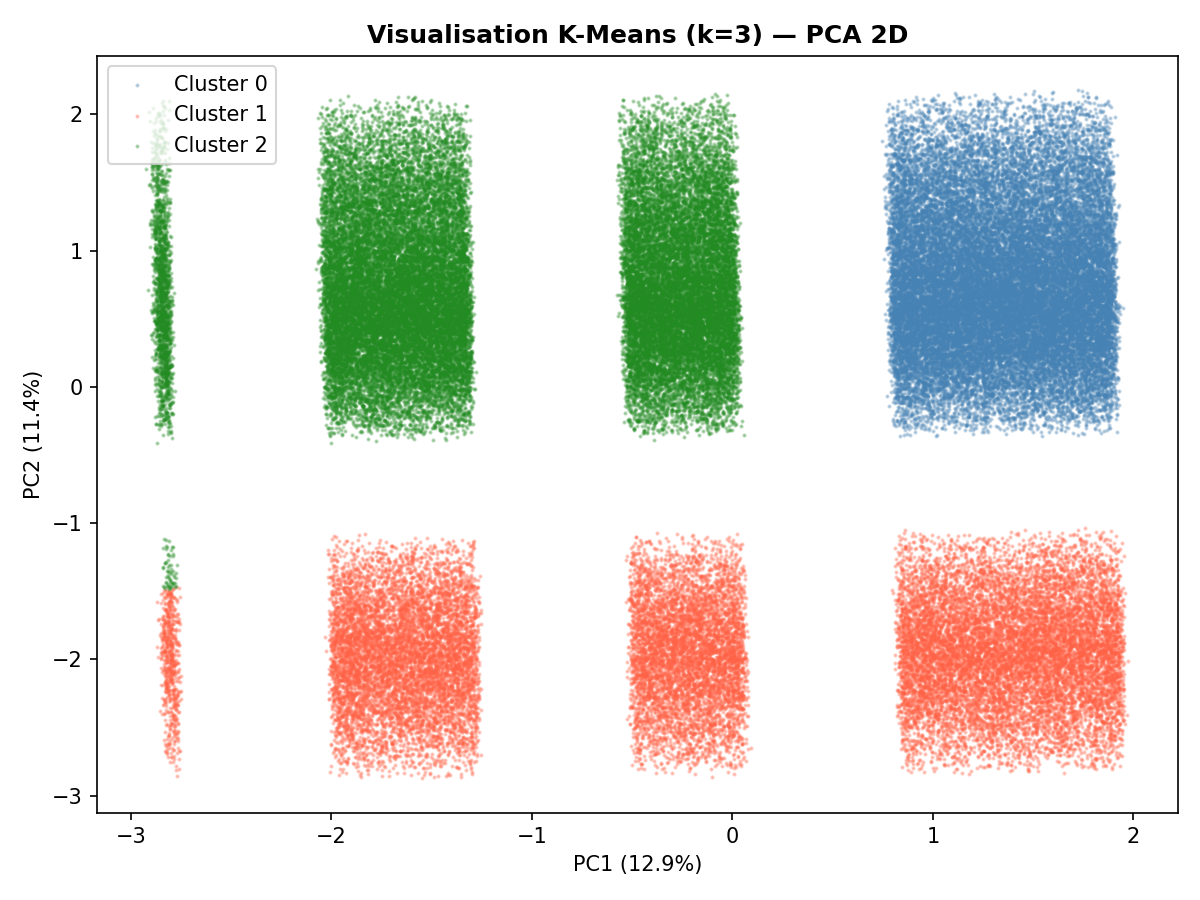
\includegraphics[width=0.85\textwidth]{kmeans_pca.png}
\caption{Visualisation des clusters K-Means ($k=3$) par projection ACP (2 composantes, 24.3\% de variance)}
\label{fig:kmeans_pca}
\end{figure}

Malgré des silhouettes faibles ($\approx 0.10$), les deux méthodes révèlent des structures interprétables médicalement~\cite{booth2012, who2000}~: obèse hypertendu (K-Means), fumeurs intenses + hypertendus (CAH). La faible silhouette reflète l'absence de groupes naturels francs dans des données synthétiques générées sans structure causale --- pas une erreur méthodologique.

% ─────────────────────────────────────────────────────────────
\section{Interprétabilité des modèles}

\subsection{Objectif}

Cette section pose une question précise~: \textbf{les outils d'interprétabilité convergent-ils vers les mêmes variables influentes, même en l'absence de signal~?} La réponse est elle-même un résultat analytique.

\subsection{Outils utilisés}

\textbf{Coefficients des modèles linéaires}~: un coefficient $w_j > 0$ indique qu'une augmentation de la variable $j$ est associée à une augmentation de la prédiction~\cite{james2021}. Leur magnitude reflète l'importance relative de chaque variable --- sous réserve que les variables soient standardisées.

\textbf{Feature Importance (impureté de Gini)}~\cite{breiman2001}~: pour les forêts aléatoires, l'importance de la variable $j$ agrège la réduction d'impureté de Gini qu'elle apporte à travers tous les nœuds de tous les arbres. Plus une variable est utilisée haut dans les arbres pour des décisions qui séparent bien les classes, plus son importance est élevée. La limite connue de cet indicateur~: il favorise les variables à haute cardinalité ou grande variance --- ce qui, dans notre cas, explique que \texttt{systolic\_bp} domine systématiquement.

\textbf{SHAP}~: défini au chapitre~1 (formule des valeurs de Shapley) et utilisé ici comme complément visuel, il attribue à chaque variable une contribution signée à chaque prédiction individuelle. Les formules ne sont pas redéfinies ici.

\subsection{Résultats, convergence et analyse critique}

Les cinq méthodes d'interprétabilité (coefficients LR, Ridge, feature importance RF, XGBoost, SHAP) sont appliquées et leurs top~5 variables comparés.

\begin{quote}
\textbf{Analyse critique~:} Les cinq méthodes ne s'accordent pas sur un classement stable~--- \textbf{cette divergence est elle-même un résultat}~\cite{rudin2019}~: sans signal prédictif réel, chaque outil mesure du bruit aléatoire et s'accroche à des corrélations parasites différentes. La seule variable présente dans les cinq méthodes est \texttt{systolic\_bp}~: dans la littérature épidémiologique réelle, la pression artérielle est effectivement l'un des facteurs de risque cardiovasculaire les mieux documentés~\cite{esc2018}~--- mais dans nos données, cette convergence résulte de sa grande variance, pas d'une vraie relation causale.

Sur des données réelles~\cite{booth2012, who2000}, on s'attendrait à voir la pression artérielle, le cholestérol LDL, le tabagisme, l'IMC et l'activité physique dominer clairement les classements, avec des coefficients significativement différents de zéro.
\end{quote}

\begin{figure}[h]
\centering
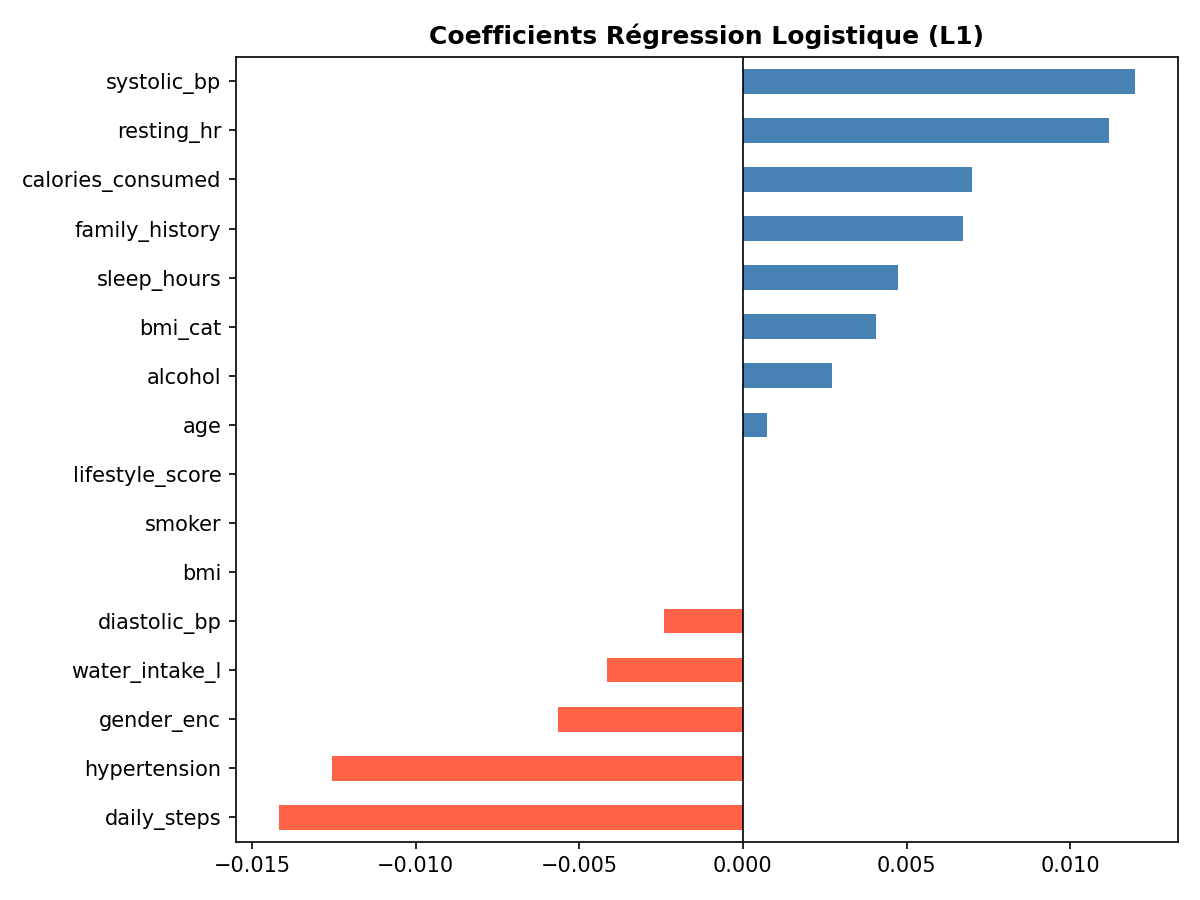
\includegraphics[width=0.75\textwidth]{lr_coefficients.png}
\caption{Coefficients de la régression logistique (variables standardisées)}
\label{fig:lr_coef}
\end{figure}

\begin{figure}[h]
\centering
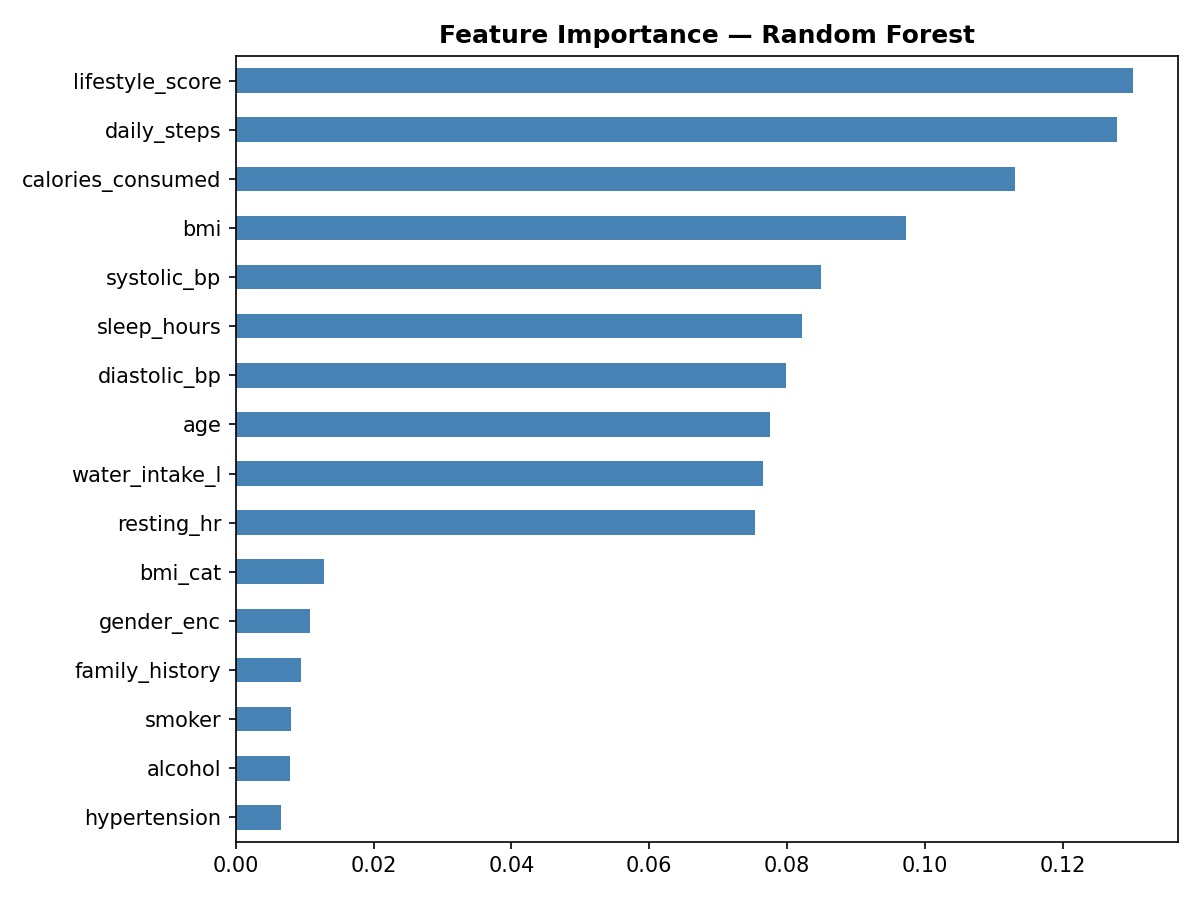
\includegraphics[width=0.75\textwidth]{rf_feature_importance.png}
\caption{Feature importances (impureté de Gini) du Random Forest}
\label{fig:rf_fi}
\end{figure}

\begin{figure}[h]
\centering
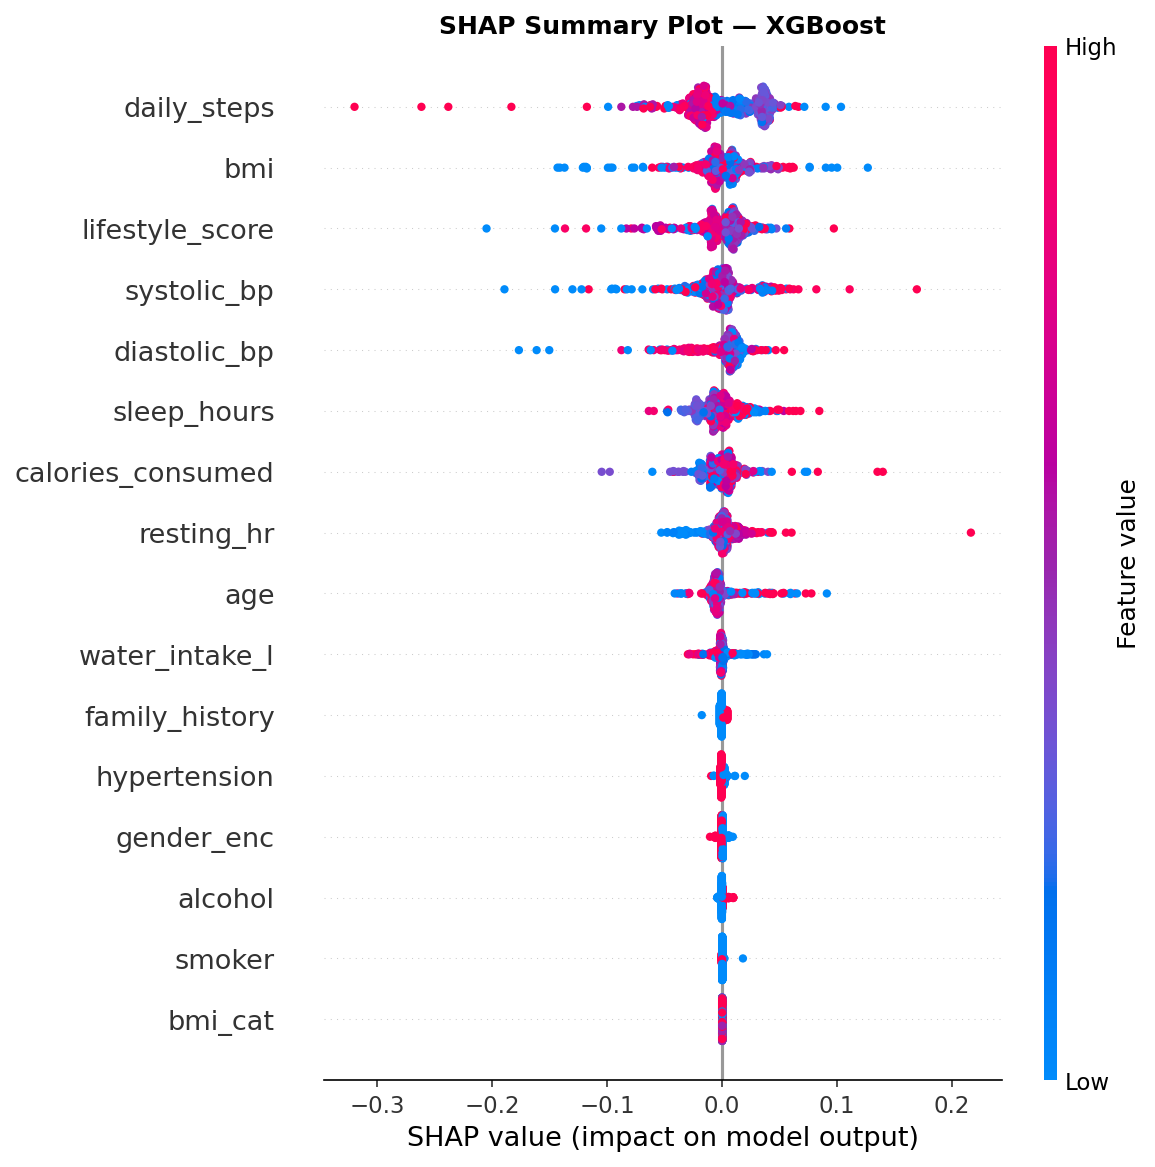
\includegraphics[width=0.85\textwidth]{shap_summary.png}
\caption{SHAP summary plot (XGBoost) --- complément visuel d'interprétabilité}
\label{fig:shap}
\end{figure}

\begin{quote}
\textbf{Comment lire le SHAP summary plot~?} Chaque \textbf{ligne} correspond à une variable, triée de haut en bas par importance décroissante (impact moyen en valeur absolue). Sur chaque ligne, chaque \textbf{point} représente un individu. L'\textbf{axe horizontal} indique l'impact SHAP sur la prédiction~: un point à droite ($x > 0$) signifie que la variable pousse la prédiction vers 1 (\texttt{disease\_risk} élevé)~; un point à gauche ($x < 0$) la pousse vers 0~; en $x = 0$, aucun impact. La \textbf{couleur} encode la valeur réelle de la variable~: rouge = valeur élevée, bleu = valeur faible.

Sur des données avec un signal réel, on verrait un gradient net~: par exemple, si une pression artérielle élevée (rouge) est un facteur de risque, les points rouges se concentreraient à droite et les bleus à gauche. Ici, les couleurs sont \textbf{mélangées aléatoirement} autour de zéro~: des points rouges et bleus occupent les mêmes positions horizontales, sans aucun pattern. Cela confirme qu'aucune variable n'a d'impact systématique~--- SHAP détecte du bruit plutôt qu'un signal.
\end{quote}

Le tableau suivant synthétise la présence de chaque variable dans le top~5 des cinq méthodes~:

\begin{table}[h]
\centering
\caption{Variables dans le top 5 de chaque méthode d'interprétabilité}
\label{tab:interpretability}
\begin{tabular}{lcccccc}
\toprule
Variable & LR & RF & XGB & SHAP & Ridge & Score \\
\midrule
\texttt{systolic\_bp}   & \checkmark & \checkmark & \checkmark & \checkmark & \checkmark & \textbf{5/5} \\
\texttt{daily\_steps}   & \checkmark & \checkmark & ---        & \checkmark & ---        & 3/5 \\
\texttt{family\_history}& \checkmark & ---        & \checkmark & ---        & \checkmark & 3/5 \\
\texttt{bmi}            & ---        & \checkmark & ---        & \checkmark & ---        & 2/5 \\
\bottomrule
\end{tabular}
\end{table}


\chapter{Organisation, retour d'expérience et perspectives}
% !TEX root = ../manuscript.tex

\section{Méthodologie et organisation}

\subsection{Approche CRISP-DM}

Ce projet a été conduit en suivant le cycle \textbf{CRISP-DM}~\cite{chapman2000}, qui structure un projet de data science en six phases~: compréhension du problème, compréhension des données, préparation des données, modélisation, évaluation, et déploiement. Chaque phase a alimenté la suivante de manière itérative~: l'EDA a révélé l'absence de signal linéaire, ce qui a orienté le choix des modèles non-linéaires~; la détection du data leakage a conduit à réviser le feature engineering~; les résultats de classification ont confirmé le diagnostic de l'EDA.

\subsection{Outils et environnement technique}

\begin{table}[h]
\centering
\caption{Stack technique du projet}
\label{tab:tech_stack}
\begin{tabular}{lll}
\toprule
Catégorie & Outil & Usage \\
\midrule
Langage              & Python 3                  & Ensemble du projet \\
Manipulation données & pandas, numpy             & Chargement, nettoyage, feature engineering \\
Modélisation         & scikit-learn, xgboost     & Entraînement, tuning, évaluation \\
Déséquilibre classes & imbalanced-learn          & Rééchantillonnage SMOTE \\
Interprétabilité     & shap                      & Valeurs SHAP sur XGBoost \\
Réduction de dim.    & scikit-learn (PCA)        & Visualisation clustering \\
Versionnement        & Git / GitHub              & Suivi des notebooks et du rapport \\
Rédaction            & \LaTeX                    & Mémoire \\
\bottomrule
\end{tabular}
\end{table}

\subsection{Compétences mobilisées}

\begin{table}[h]
\centering
\caption{Lien entre enseignements MIASHS et applications projet}
\label{tab:competences}
\begin{tabular}{ll}
\toprule
Enseignement M1 & Application dans le projet \\
\midrule
ACP / ACM                          & Réduction dimensionnelle pour la visualisation des clusters \\
Régression linéaire \& diagnostic  & Baseline régression, Ridge, Lasso, ElasticNet \\
Classification supervisée          & Logistic Regression, Random Forest, XGBoost \\
Apprentissage non supervisé        & K-Means, CAH \\
Descente de gradient \& optimisation & Compréhension de XGBoost et de la log-loss \\
Régression logistique              & Baseline classification + interprétation coefficients \\
Régularisation \& optimisation     & Ridge, Lasso, ElasticNet \\
Déséquilibre de classes            & class\_weight, SMOTE (imbalanced-learn) \\
Python                             & Ensemble du pipeline de data science \\
\bottomrule
\end{tabular}
\end{table}

\section{Difficultés rencontrées et retour d'expérience}

\subsection{Difficultés techniques}

\textbf{La limite fondamentale du dataset synthétique} est la difficulté principale que j'ai rencontrée. Découvrir que $R^2 \approx 0$ et AUC $\approx 0.5$ pour tous les modèles a demandé un vrai travail de diagnostic~: relier ce résultat au constat de l'EDA (corrélations $< 0.01$) et à la nature synthétique des données a été l'exercice analytique central de ce projet.

\textbf{La détection du data leakage} sur \texttt{hypercholesterol}~\cite{kaufman2012} est une difficulté classique en ML, rarement rencontrée dans les travaux académiques. Le $R^2$ artificiel de 0.675 aurait pu passer inaperçu sans une analyse rigoureuse des feature importances.

\textbf{Le coût computationnel}~: un premier essai de Random Forest sans \texttt{max\_depth} ni \texttt{n\_jobs=-1} a conduit à un entraînement de plus de 3 heures interrompu avant convergence. Ça m'a forcé à comprendre les paramètres internes de l'algorithme. Le SVM a été écarté pour la même raison, sa complexité en $\mathcal{O}(n^2)$ étant incompatible avec 100~000 observations.

\subsection{Compétences acquises}

\begin{itemize}
  \item \textbf{Détection et correction du data leakage}~\cite{kaufman2012}~: piège courant non systématiquement couvert en cours théoriques.
  \item \textbf{RandomizedSearchCV}~\cite{bergstra2012}~: logique de l'exploration aléatoire vs exhaustive des hyperparamètres.
  \item \textbf{Gestion du déséquilibre de classes}~: comparaison concrète entre \texttt{class\_weight='balanced'} et SMOTE~\cite{chawla2002}, et compréhension de la différence entre accuracy, F1-score et AUC-ROC~\cite{sokolova2009}.
  \item \textbf{Interprétabilité multi-méthodes}~: la divergence entre outils est elle-même informative~\cite{rudin2019}.
  \item \textbf{Analyse critique d'un résultat négatif}~: savoir diagnostiquer pourquoi un modèle échoue est aussi précieux que d'en construire un qui réussit.
\end{itemize}

\subsection{Plus-value~: diagnostiquer les biais du pipeline}

Ce projet ne produit pas un modèle prédictif déployable --- les métriques ($R^2 \approx 0$, AUC $\approx 0.5$) l'excluent. Sa plus-value réside dans une contribution différente~: \textbf{construire un pipeline capable de diagnostiquer pourquoi un modèle échoue}, et d'identifier rigoureusement ses biais.

Trois apports concrets peuvent être retenus~:

\begin{enumerate}
  \item \textbf{Détection du data leakage.} La variable \texttt{hypercholesterol} produisait un $R^2$ artificiel de 0.675~\cite{kaufman2012}. Un pipeline mal construit aurait publié ce résultat comme une performance réelle. La détection et la correction rigoureuse de ce biais est une compétence directement valorisable sur des données épidémiologiques réelles.

  \item \textbf{Diagnostic de l'absence de signal par cinq preuves convergentes.} Corrélations de Pearson $< 0.01$ (EDA), $R^2 \approx 0$ sur six modèles de régression dont des méthodes non-linéaires (Random Forest, XGBoost), AUC $\approx 0.5$ sur trois modèles de classification, silhouettes $\approx 0.10$ en clustering, et divergence des cinq outils d'interprétabilité. Cette convergence de preuves indépendantes est plus robuste qu'un résultat isolé.

  \item \textbf{Accuracy trompeuse sur données déséquilibrées.} Un modèle naïf atteignait 75\% d'accuracy sur le déséquilibre 75/25~; le Random Forest affichait 56.8\% d'accuracy mais une AUC de 0.494, soit \textit{pire} que le hasard pur~\cite{sokolova2009}. Identifier et exposer ce piège méthodologique est un résultat analytique à part entière.
\end{enumerate}

Ce pipeline est \textbf{directement transposable} sur des données réelles~\cite{dawber1951, nhanes}~: les mêmes étapes de détection de leakage, de validation des métriques et de comparaison des méthodes s'appliquent, et le signal réel permettrait d'obtenir des résultats prédictifs exploitables.

\subsection{Biais identifiés et enjeux éthiques}

Au-delà du data leakage --- biais technique identifié et corrigé --- ce projet met en évidence des biais plus fondamentaux, de nature méthodologique et éthique, qu'il est nécessaire d'analyser explicitement.

\textbf{1. Biais de représentation~: l'impossibilité de généraliser.} Le dataset est synthétique~: les 100~000 individus ne représentent aucune population réelle. Les distributions ont été générées sans ancrage épidémiologique validé (aucune cohorte de référence, aucun rapport sur la méthode de génération). Cela rend toute généralisation structurellement impossible~: un modèle entraîné ici ne peut pas être évalué sur Framingham~\cite{dawber1951} ou NHANES~\cite{nhanes}, car les distributions diffèrent de façon inconnue. Ce biais est antérieur à toute modélisation~: il est inscrit dans le choix du dataset.

\textbf{2. Biais de conception~: répondre à une question avec des données inadaptées.} L'objectif initial est de modéliser les relations entre habitudes de vie et indicateurs biologiques. Or, dans un dataset synthétique sans structure causale, les variables ont été générées indépendamment~: il n'existe, par construction, aucune relation à découvrir~\cite{scholkopf2021}. Appliquer des méthodes de ML sur ces données revient à chercher un signal que l'on sait absent. Ce biais de conception est distinct du biais de représentation~: même si le dataset représentait une vraie population, l'absence de structure causale rendrait l'inférence impossible. En termes d'apprentissage causal~\cite{pearl2009}, le DAG sous-jacent est un graphe sans arcs --- chaque variable est une île.

\textbf{3. Enjeux de fairness algorithmique.} Si ce pipeline était déployé sur des données réelles, un biais critique émergerait~: les performances peuvent varier considérablement selon les sous-groupes. Le travail d'Obermeyer et al.~\cite{obermeyer2019} a démontré qu'un algorithme utilisé dans des millions d'hôpitaux américains présentait un biais racial systématique, pénalisant les patients noirs à sévérité médicale égale. En santé, la fairness n'est pas un aspect secondaire~: un modèle avec AUC globale acceptable peut masquer des performances très inégales selon le genre, l'âge, ou d'autres attributs protégés~\cite{rudin2019}. Dans ce projet, le déséquilibre 75/25 sur \texttt{disease\_risk} est lui-même un signal~: si cette variable était réelle, le seuil de décision du classificateur devrait être calibré en tenant compte de l'impact différentiel sur les groupes sous-représentés.

\textbf{4. Risques de déploiement~: quand l'absence de signal devient dangereuse.} Un résultat central de ce projet --- AUC $\approx 0.5$ --- signifie que les modèles ne font pas mieux que le hasard pour prédire \texttt{disease\_risk}. Ce résultat, s'il était mal interprété ou ignoré, pourrait conduire à des décisions erronées. Un praticien ou un décideur qui fait confiance à un modèle avec AUC = 0.494 prend des décisions au hasard, avec en plus l'illusion d'une base scientifique. Cette situation --- modèle inutile mais présenté comme fiable --- est l'un des risques les plus documentés de l'IA en santé~\cite{rajpurkar2022}. La calibration des prédictions (est-ce que "70\% de probabilité de risque" en sortie correspond vraiment à 70\% de cas réels~?) est une exigence minimale avant tout déploiement.

Ces quatre biais --- représentation, conception, fairness, déploiement --- constituent l'essentiel du travail critique qu'un data scientist doit conduire avant de présenter des résultats, y compris des résultats négatifs. Les identifier n'invalide pas le projet~: cela en précise le périmètre de validité et les conditions d'un travail de suivi crédible.

\subsection{Positionnement RSE / DDRS}

L'utilisation d'un dataset \textbf{synthétique} s'inscrit dans une démarche éthique~: les données de santé sont sensibles et encadrées par le RGPD~\cite{rgpd2016}. Les données synthétiques éliminent tout risque de ré-identification tout en permettant de développer des méthodes~--- un compromis central de l'IA responsable~\cite{rgpd2016}.

Le coût énergétique des entraînements a été limité en contraignant la profondeur des arbres (\texttt{max\_depth=15}) et en réduisant \texttt{n\_iter} dans \texttt{RandomizedSearchCV}, avec un impact positif sur l'empreinte carbone du calcul.

\subsection{Limites méthodologiques}

\textbf{Corrélations non-linéaires non explorées.} L'analyse de Pearson a révélé des coefficients inférieurs à $|0.01|$ --- mais Pearson ne détecte que les relations \textit{linéaires}~\cite{james2021}. Une analyse complémentaire aurait pu mobiliser le coefficient de Spearman (corrélation des rangs, capte les relations monotones), la \textit{mutual information} (\texttt{mutual\_info\_classif} dans scikit-learn, toute dépendance statistique quelle que soit sa forme), ou des nuages de points pour identifier visuellement des structures non-linéaires (relations en U, effets seuil, interactions).

Toutefois, l'utilisation de \textbf{Random Forest et XGBoost}~\cite{breiman2001} --- algorithmes capables de capturer n'importe quelle relation non-linéaire --- constitue une réponse indirecte à cette limite. Leur échec ($R^2 \approx 0$, AUC $\approx 0.5$) démontre que même les dépendances non-linéaires sont absentes~: résultat plus fort qu'un test de Spearman ou de mutual information, car il exploite toute la puissance des méthodes ensemblistes sur 100~000 individus.

\section{Perspectives}

\textbf{1. Changer de dataset}~: reproduire le pipeline sur un dataset réel, comme la cohorte Framingham~\cite{dawber1951} ou les données NHANES~\cite{nhanes}, qui contiennent de vraies relations entre habitudes de vie et indicateurs de santé. Les méthodes développées ici sont directement transposables.

\textbf{2. Améliorer les modèles de classification}~: explorer le \textbf{stacking} (combinaison de plusieurs modèles~\cite{hastie2009}) et les \textbf{réseaux de neurones} pour capturer des relations très non-linéaires~--- en lien direct avec le module Deep Learning du master. SMOTE ayant déjà été intégré dans ce projet, ces pistes constituent la suite logique.

\textbf{3. Déploiement}~: un modèle de classification pourrait être déployé sous forme d'API REST (FastAPI) permettant de soumettre un profil individuel et d'obtenir une prédiction avec ses valeurs SHAP associées, rendant le modèle accessible et explicable.

\textbf{4. Interprétabilité avancée}~: les \textit{Partial Dependence Plots} (PDP) et les \textit{Individual Conditional Expectation} (ICE) permettraient de visualiser comment la prédiction varie en fonction d'une variable, toutes choses égales par ailleurs~--- une limite de SHAP qui agrège les contributions.

\textbf{5. Robustesse sur le long terme (\textit{data drift})~:} sur des données réelles en production, un modèle se dégrade si la distribution des données évolue au fil du temps~--- on parle de \textit{concept drift}~\cite{hastie2009}. Les habitudes de vie d'une population changent, les seuils médicaux sont révisés, les profils épidémiologiques se transforment. En pratique, cela implique de surveiller les performances du modèle périodiquement (suivi de l'AUC sur de nouvelles cohortes) et de le réentraîner dès que les performances se dégradent. Cette problématique ne s'applique pas au dataset synthétique statique de ce projet, mais sera centrale sur des données réelles.

\textbf{6. Vers le Master 2}~: les thématiques de causalité, fairness algorithmique et apprentissage fédéré constituent des pistes naturelles pour un travail de recherche en M2, dans la continuité directe de ce projet.


\addstarredchapter{Conclusion}
% !TEX root = ../manuscript.tex
\clearpage

Ce projet a mobilisé un pipeline complet de data science --- analyse exploratoire, feature engineering, régression, classification, clustering et interprétabilité --- appliqué à un jeu de données de santé et de mode de vie de 100~000 individus. La question centrale était~: \textit{quels facteurs de mode de vie influencent le plus l'état de santé d'un individu, et peut-on les modéliser de manière fiable et interprétable~?}

La réponse est double. \textbf{Du point de vue des résultats}~: ce dataset synthétique ne permet pas de répondre à cette question --- les variables ont été générées indépendamment, sans relation causale encodée. Aucun modèle, linéaire ou non-linéaire, simple ou optimisé, n'a dépassé les performances d'un prédicteur naïf ($R^2 \approx 0$, AUC $\approx 0.5$). Cette découverte progressive est elle-même un résultat analytique~: elle illustre concrètement la différence entre données synthétiques et données réelles, et la nécessité d'interroger la qualité du signal avant de construire des modèles.

\textbf{Du point de vue méthodologique}~: chaque étape du pipeline a été conduite avec rigueur. L'EDA a permis d'anticiper les difficultés. La détection d'un data leakage~\cite{kaufman2012} a évité une surestimation artificielle des performances. La comparaison systématique de six modèles avec tuning par \texttt{RandomizedSearchCV}~\cite{bergstra2012} et validation croisée stratifiée a respecté les bonnes pratiques d'évaluation. L'analyse d'interprétabilité multi-méthodes a montré que la divergence entre outils est elle-même informative~\cite{rudin2019}.

Ce projet démontre ce que signifie travailler en data scientist~: ne pas se contenter de faire tourner des algorithmes, mais comprendre ce que les données peuvent --- et ne peuvent pas --- dire. Comme le formule Rudin~\cite{rudin2019}, un bon modèle prédictif ne vaut rien sans une évaluation honnête de ses limites. Cette posture critique, à l'intersection des mathématiques, de la statistique et de l'informatique appliquée, est au c\oe ur de la formation MIASHS.

Les perspectives identifiées --- notamment l'application de ce pipeline sur des données épidémiologiques réelles comme les cohortes Framingham~\cite{dawber1951} ou NHANES~\cite{nhanes} --- ouvrent des directions concrètes pour un travail de recherche en Master~2, avec l'ambition d'obtenir des modèles à la fois performants, interprétables et éthiquement responsables~\cite{floridi2019}.


\addstarredchapter{Bibliographie}
\bibliographystyle{unsrt}
\bibliography{references}

\addstarredchapter{Liste des abréviations}
% !TEX root = ../manuscript.tex

\begin{tabular}{@{}ll}
\textbf{ACP}      & Analyse en Composantes Principales \\
\textbf{AUC}      & Area Under the Curve \\
\textbf{CAH}      & Classification Ascendante Hiérarchique \\
\textbf{EDA}      & Exploratory Data Analysis (Analyse Exploratoire des Données) \\
\textbf{ESC}      & European Society of Cardiology \\
\textbf{FE}       & Feature Engineering \\
\textbf{IMC}      & Indice de Masse Corporelle \\
\textbf{MAE}      & Mean Absolute Error (Erreur Absolue Moyenne) \\
\textbf{MIASHS}   & Mathématiques et Informatique Appliqués aux Sciences Humaines et Sociales \\
\textbf{ML}       & Machine Learning \\
\textbf{NCEP}     & National Cholesterol Education Program \\
\textbf{OMS}      & Organisation Mondiale de la Santé \\
\textbf{RMSE}     & Root Mean Squared Error (Racine de l'Erreur Quadratique Moyenne) \\
\textbf{ROC}      & Receiver Operating Characteristic \\
\textbf{SHAP}     & SHapley Additive exPlanations \\
\textbf{SMOTE}    & Synthetic Minority Over-sampling Technique \\
\textbf{SVM}      & Support Vector Machine \\
\textbf{WHO}      & World Health Organization \\
\end{tabular}

\newpage


\addstarredchapter{Lexique}
% !TEX root = ../manuscript.tex

\begin{description}
  \item[\textbf{Clustering}] Méthode d'apprentissage non supervisé visant à regrouper des observations similaires sans variable cible prédéfinie.

  \item[\textbf{Cross-validation (validation croisée)}] Technique d'évaluation qui consiste à diviser les données en $k$ sous-ensembles et à entraîner/tester le modèle $k$ fois.

  \item[\textbf{Data leakage}] Fuite d'information du jeu de test vers le jeu d'entraînement, entraînant une surestimation artificielle des performances.

  \item[\textbf{Feature engineering}] Processus de création ou de transformation de variables à partir des données brutes pour améliorer les performances des modèles.

  \item[\textbf{Feature importance}] Mesure de la contribution de chaque variable à la prédiction d'un modèle.

  \item[\textbf{Hyperparamètre}] Paramètre d'un modèle fixé avant l'entraînement (ex.~: $\lambda$ pour Ridge, $k$ pour K-Means).

  \item[\textbf{Overfitting (surapprentissage)}] Phénomène où un modèle apprend trop précisément les données d'entraînement et généralise mal sur de nouvelles données.

  \item[\textbf{Pipeline}] Enchaînement structuré d'étapes de traitement des données et de modélisation.

  \item[\textbf{Régularisation}] Technique pénalisant la complexité d'un modèle pour réduire l'overfitting (ex.~: Ridge $L_2$, Lasso $L_1$).

  \item[\textbf{SHAP}] Méthode d'interprétabilité basée sur la théorie des jeux coopératifs, attribuant à chaque variable une contribution marginale à la prédiction.

  \item[\textbf{Silhouette}] Coefficient mesurant la qualité d'un clustering~: proche de 1 si les clusters sont bien séparés, proche de 0 s'ils se chevauchent.

  \item[\textbf{SMOTE}] Technique de rééchantillonnage qui génère synthétiquement des exemples de la classe minoritaire pour corriger le déséquilibre des classes.

  \item[\textbf{Tuning}] Processus d'optimisation des hyperparamètres d'un modèle, souvent via une recherche aléatoire ou par grille.
\end{description}

\newpage


\addstarredchapter{Annexes}
% !TEX root = ../manuscript.tex

\section*{Annexe A — Variables du dataset}

\begin{longtable}{@{}llll@{}}
\toprule
\textbf{Variable} & \textbf{Type} & \textbf{Description} & \textbf{Unité / Modalités} \\
\midrule
\texttt{age}              & Continue  & Âge de l'individu                        & années \\
\texttt{bmi}              & Continue  & Indice de masse corporelle                & kg/m² \\
\texttt{daily\_steps}     & Continue  & Nombre de pas quotidiens                  & pas/jour \\
\texttt{sleep\_hours}     & Continue  & Durée de sommeil                          & heures/nuit \\
\texttt{water\_intake\_l} & Continue  & Consommation d'eau                        & litres/jour \\
\texttt{calories\_consumed}& Continue & Apport calorique quotidien                & kcal/jour \\
\texttt{smoker}           & Binaire   & Statut tabagique                          & 0 = non, 1 = oui \\
\texttt{alcohol}          & Binaire   & Consommation d'alcool                     & 0 = non, 1 = oui \\
\texttt{resting\_hr}      & Continue  & Fréquence cardiaque au repos              & bpm \\
\texttt{systolic\_bp}     & Continue  & Pression artérielle systolique            & mmHg \\
\texttt{diastolic\_bp}    & Continue  & Pression artérielle diastolique           & mmHg \\
\texttt{cholesterol}      & Continue  & Taux de cholestérol total                 & mg/dL \\
\texttt{family\_history}  & Binaire   & Antécédents familiaux de maladie          & 0 = non, 1 = oui \\
\texttt{gender}           & Catégorielle & Sexe de l'individu                     & Male / Female \\
\texttt{disease\_risk}    & Binaire   & Variable cible : risque de maladie        & 0 = non, 1 = oui \\
\bottomrule
\end{longtable}

\newpage

\section*{Annexe B — Hyperparamètres testés (RandomizedSearchCV)}

\begin{longtable}{@{}lll@{}}
\toprule
\textbf{Modèle} & \textbf{Hyperparamètre} & \textbf{Valeurs explorées} \\
\midrule
Ridge         & \texttt{alpha}                  & $[0.01, 0.1, 1, 10, 100]$ \\
Lasso         & \texttt{alpha}                  & $[0.001, 0.01, 0.1, 1, 10]$ \\
ElasticNet    & \texttt{alpha}, \texttt{l1\_ratio} & $[0.01\text{--}10]$, $[0.1, 0.5, 0.9]$ \\
Random Forest & \texttt{n\_estimators}, \texttt{max\_depth} & $[50, 100, 200]$, $[5, 10, 15]$ \\
XGBoost       & \texttt{learning\_rate}, \texttt{n\_estimators} & $[0.01, 0.05, 0.1]$, $[100, 200]$ \\
\bottomrule
\end{longtable}

\newpage


\end{document}
